
\section{Results}
\label{sec:result}

\subsection{LHC Procedure For Limits Setting}
\label{sec:limits}
A detailed description of the LHC procedure for Higgs search can be found in \cite{lhc,cramer},
in the following a brief summary is given.
Statistical tests are used for quantify an observation or to set an exclusion limit, 
in search for new phenomena, hypotesis testing is performed by means of two hypotesis: 
the \textit{background only} $H_0$ and and the \textit{signal+background} $H_1$.  
As its has allready been outlined in section~\ref{sec:stat1}, any statistical test is based on probability
distribution, once a probability density function (p.d.f.) is defined, one can calculate its value for a given 
set of data obtaining what is called a "likelihood".  Taking the marked Poisson
p.d.f. in equation~\eqref{markedpoisson}  one obtain the following likelihood function:
\begin{equation}\label{likelihood}
\mathcal{L}(\text{data}|\mu, \boldsymbol{\theta}) = \text{Poisson(data} | \mu \cdot s(\boldsymbol{\theta}) + b(\boldsymbol{\theta})) 
	\cdot f(\boldsymbol{\theta} | \hat{\boldsymbol{\theta}})
\end{equation}
this now describes how likely are the data under a certain hypotesis and it is only function of the parameter $\mu$ and of the
nuissance parameter $\boldsymbol{\theta}$. If the hypotesis under test is unlikely to happen with the given dataset the value of 
$\mathcal{L}$ is decreasing,
one can define which is the best value of a parameter that describes the data via maximising the likelihood,
obtaining a so called maximum likelihood estimator. The Poisson distribution in equation~\eqref{likelihood}
stands for a product of Poisson probabilities to observe  events in the bin \textit{i} of an histogram:
$$
\prod_{i} \frac{(\mu s_i +b_i)^{n_i}}{n_i!} ~ e^{-\mu s_i -b_i}
$$
while the $f(\boldsymbol{\theta} | \hat{\boldsymbol{\theta}})$ is the p.d.f. for a given set of nuissance 
parameter $\boldsymbol{\theta}$ with their best estimate $\hat{\boldsymbol{\theta}}$. 

\begin{figure}[tp]
  \centering
 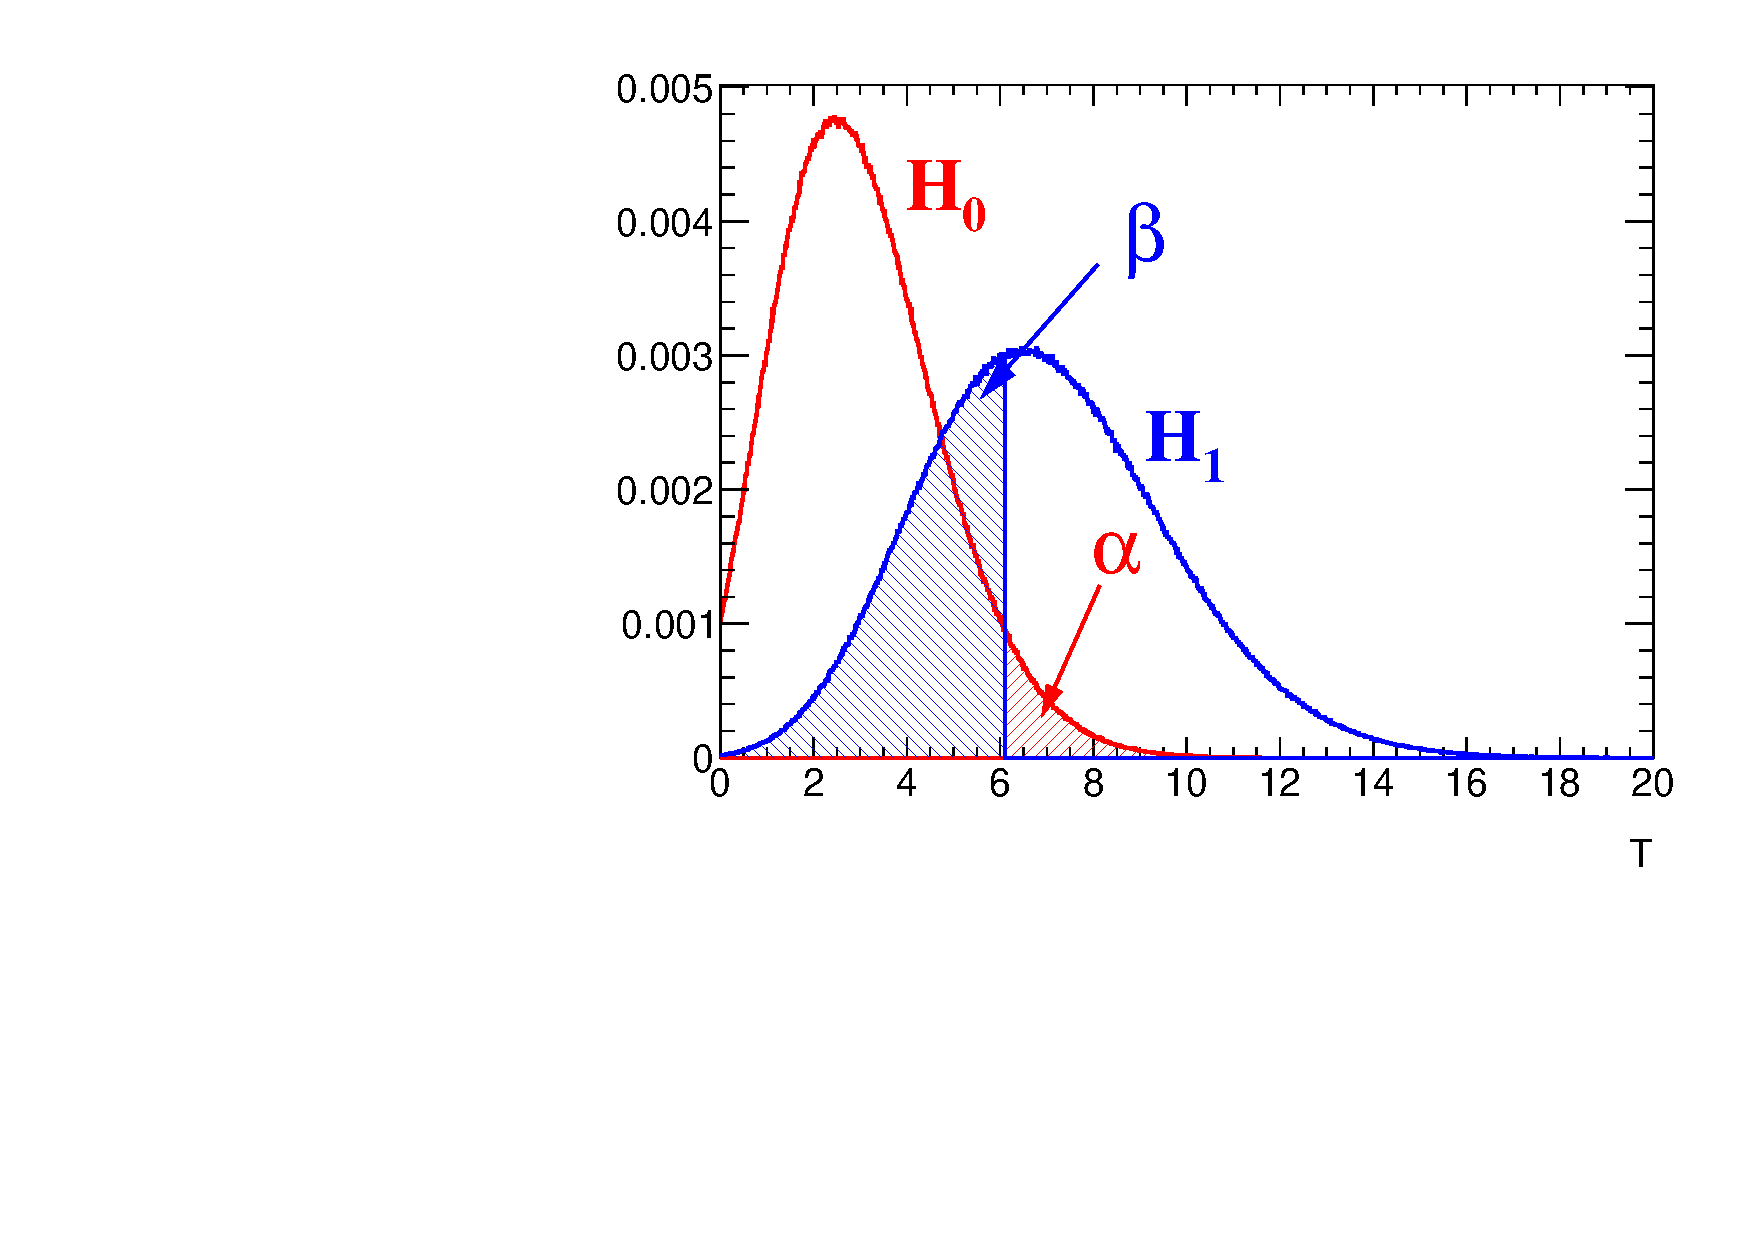
\includegraphics[width=0.5\textwidth]{figure/test_stat.pdf}
  \caption{Example of a test statistic which in this case is just the total number of events of a counting experiment.
	Under the hypotesis $H_0$ are expected four events, while under the $H_1$ seven  events are expected.} 
\label{fig:teststat}
\end{figure}

To compiute the compatibility of the data with the $H_{0}$ and $H_{1}$ hypotesis and then exclusion limits, 
one needs to define a test statistic. The test statistic, which has already been mentioned in section~\ref{sec:stat1},
is a function of the data which returns a real value. One can in principle use any test statistic, however, 
given the size of the test (probability to reject the null hypotesis when is true) one would like to have 
a test statistic which has the highest power $1 - \beta$ possible (probability to reject the 
null hypotesys when it is false). Figure~\ref{fig:teststat} shows an example
of the distribution of an hipotetical test statistic for two hypotesis.
It has been shown by Neuman-P~\cite{} that in case of simple hyptesis (probability model without any parameter),
then the test statistic with the highest power is the ratio of the likelihood calculated with the two hypotesis.
The standard procedure at the LHC is to use the following test statistic \cite{} based on the likelihood ratio:
$$
\tilde{q_{\mu}} ~ = ~ -2 \text{ln} ~ \frac{\mathcal{L}(\text{data}|\mu, \hat{\boldsymbol{\theta}}_{\mu})}{\mathcal{L}(\text{data}|\hat{\mu}, \hat{\boldsymbol{\theta}})}
\quad \text{with the constraint} \quad 0 \leq \hat{\mu} \leq \mu
$$
 where $\hat{\mu}$ and $\hat{\boldsymbol{\theta}}$ are the maximum likelihood estimators for $\mu$ and $\boldsymbol{\theta}$ given the data, 
whereas $\hat{\boldsymbol{\theta}}_{\mu}$ is the maximul likelihood estimator of $\boldsymbol{\theta}$ given the data but considering
a signal streght of value $\mu$, $\tilde{q_{\mu}}$ is increasing with increasing disagreement between data and the $\mu$ hypotesis under test.
The procedure for limits setting follows five steps:
\begin{enumerate}
	\item The signal hypotesis with signal streght $\mu$ is assumed, under this assumpion a set of 
	\textit{pseudo-data} is generated for different values of $\mu$.

	\item  $\tilde{q_{\mu}}$ is calculated for each of the \textit{pseudo-dataset} and each signal hypotesis generating
	the expected probability density function for $\tilde{q_{\mu}}$ given $\mu$, 
	$\text{f}(\tilde{q_{\mu}} ~| ~ \mu, \hat{\boldsymbol{\theta}}_{\mu},H_1)$.

	\item One does the same thing for the null hypotesis, generate pseudo-data with the distribution of background only and 
	obtain  the $\text{f}(\tilde{q_{\mu}} ~ | ~ \mu = 0, \hat{\boldsymbol{\theta}}_{0}, H_0)$.

	\item Once the p.d.f. for the signal and signal + background hypotesis is obtained, one can define for a given dataset (that can be this time
	real data or again pseudodata)  two p-values for any given value of $\mu$, which are the probability to obtain data less compatible with the hypotesis in consideration:
	$$
	p_{s+b} = P(\tilde{q_{\mu}} > \tilde{q_{\mu}}^{observed} ~ | ~ H_1)  
	$$
	$$ 
	p_{b} = P(\tilde{q_{\mu}} > \tilde{q_{\mu}}^{observed} ~ | ~ H_0)
	$$
	The ratio of this two probability is what is called the $CL_{s} = p_{s+b} / p_{b}$ \cite{}.

	\item If for a given $\mu$ is obtained $CL_{s} ~ \leq ~ \alpha $ one states that the signal hypotesis (with that $\mu$) 
	is excluded with (1 - $\alpha$) $CL_{s}$ confidence level. To get the 95\% confidence level upper limit on $\mu$,
	denoted as $\mu^{95}$ one adjust $\mu$ until $CL_{s} = 0.05$. 
\end{enumerate}
This is a quite complicated prescription, however 
its interpretation is not so different from the usual Neyman Costruction~\cite{} of confidence intervals:
for each $\mu$ is possible to define $\tilde{q_{\mu}}^{95}$ for which the probability 
P$(\tilde{q_{\mu}} \geq \tilde{q_{\mu}}^{95} ~ |~ \mu, ~ H_1$) = 5\%, this means that if $H_1$ is true one expects 
$\tilde{q_{\mu}} \geq \tilde{q_{\mu}}^{95}$ in 5\% of the cases. With this definition $\mu^{95}$ would be the value of $\mu$
that for the observed data gives $\tilde{q_{\mu}} = \tilde{q_{\mu}}^{95}$, or in other words a p-value of 5\%.
By costruction, rejecting $\mu > \mu^{95}$ the hypotesis $H_1$ will be rejected, when is true, at most 5\% of the time,
given the fact that $\tilde{q_{\mu}}$ is increasing with increasing discrepancy of the hypotesis with data.
The difference with the $CL_{s}$ prescription is that there the ratio of p-values is used to define $\mu^{95}$: 
it has been shown that this choice protect the upper limit from down fluctuation of the data, giving a conservative
estimate in any case.
%
% For each pseudo-data sample one can calculate then $\mu^{95}$, which is the biggest value of $\mu$ which gives $\tilde{q_{\mu}} > \tilde{q_{\mu}}^{95}$
%
% Generate a large set of pseudo-data under the hypotesis $H_{0}$ and calculate  $\mu^{95}$ for each of them, by costruction one would have
%	that if $H_1$ is true for $\mu > \mu^{95}$ one has $\tilde{q_{\mu}} > \tilde{q_{\mu}}^{95}$ only 5\% of the cases.
%	
%So one it is said that the $\mu > \mu^{95}$ are excluded by data under the hypotesis $H_1$ at 95\% of Confidence Level, meaning that 
%for value of $\mu > \mu^{95}$  one would reject the $H_1$ when is true at most 5\% of the time. 
%

The expected median exclusion upper-limit and its error are evaluated by generating a large sample of \emph{bacground only}
pseudo-data and calculating $CL_s$ and $\mu^{95}$ for each of them, from the distribution of  $\mu^{95}$ one can get the mean
excluded value and its error.

%How ABCD  is actually implemented in limits machinery
The actual implementation in the limit framework of the ABCD method follows that suggested in~\cite{ABCD}.
Here three free parameters are fitted: number of multi-jet events in region B, $N_{B}^{QCD}$, factor that extrapolates from SS region to OS regions, \rqcd, and the factor that 
extrapolates from isolated to anti-isolated regions $R_{BD}$. Neglecting signal contributions, the following 
equations can be written for the event yield of the B,C and D control regions:
%$$N_{B} = N_{B}^{BKG} + N_{B}^{QCD} $$ 
%$$N_{C} = N_{C}^{BKG} +  N_{B}^{QCD} \times \rqcd \times R_{BD} $$
%$$N_{D} =  N_{D}^{BKG} + N_{B}^{QCD} \times  R_{BD} $$
\begin{itemize}
\item[] $N_{B} = N_{B}^{BKG} + N_{B}^{QCD}$
\item[] $N_{C} = N_{C}^{BKG} +  N_{B}^{QCD} \times \rqcd \times R_{BD} $
\item[] $N_{D} =  N_{D}^{BKG} + N_{B}^{QCD} \times  R_{BD} $
\end{itemize}
where $N^{BKG}$ represent the prediction of  non-QCD background in the relative regions.
The estimate of multi-jet event yield in SR will be then $ N_{B}^{QCD} \times \rqcd $. This method is 
particularly powerful because in the best fit of \rqcd the statistical 
and systematics uncertainty for non-QCD backgrounds and data will be considered.


\subsection{Exclusion Limits}
The procedure described in section~\ref{sec:limits} is  the one used for the SM Higgs, for the MSSM further complication
arises: one has to consider in the signal 
model three Higges, in a particular scenario the masses and cross section are defined for a given point in the $\tan \beta - m_A$
plane, so the procedure described previously has to be repeated for each point in that plane. 
%For a given scenario, 
%a point in the  $\tan \beta - m_A$ plane is excluded with 95\% $CL_{s}$ confidence level if $\mu^{95} \leq 1$ for that point. 
%Only a limited number of $\tan \beta - m_A$ points are gerated, 
%a linear interpolation is used to determine the $\tan \beta$ excluded for a given $m_A$.
For the $m_h^{max}$ scenario exclusion limits are derived by calculating $95\%$ CLs limits on the cross section of
$bb$/$gg\to A$/$H$/$h\to\tau_{lep}\tau_{lep}$ for 15 tan$\beta$ values (between\footnote{The set of  tan$\beta$ values used
is 5, 8, 10, 13, 16, 20, 23, 26, 30, 35, 40, 45, 50, 55, 60}  $\mathrm{tan}\beta=5$ and $\mathrm{tan}\beta=60$),
a point in the  $\tan \beta - m_A$ plane is excluded if $\mu^{95} \leq 1$ for that point, 
a linear interpolation is used to determine the $\tan \beta$ excluded for a given $m_A$.
The procedure is followed for a set of different CP-odd Higgs masses $m_A$: 90, 100, 110, 120, 125, 130,
140, 150, 170, 200, 250 and 300 GeV.
The event yield has been compared between data and background expectation in bins of the \mmc distribution. The bin sizes were chosen
such that there are enough events left for the asymptotic approximation \cite{CCGV} to  hold.
Table~\ref{table:final_numbers} compares yields between data and background model for the two categories at the final
stage of the cut flow. Additionally, figure \ref{fig:mmc_categories} shows the \mmc distributions for the full b-tag and b-veto categories. 

\begin{table} [t]
\centering
\begin{tabular}{c p{0.5cm} r l l p{1cm} r l l }
\hline
\hline
Sample 	&	& \multicolumn{3}{c}{b-tag category} 		&	& \multicolumn{3}{c}{b-veto category} 		\\ 	[0.5ex]
		&	&  N(event)	&	Stat.	&Syst.  & 	&  N(event)	&  Stat.	& Syst.		\\ [0.5ex]	
\hline
\Ztautau        &     	&       418  	&    $\pm$ 6	&	&       & 54680		& $\pm$ 60	&  		\\   [0.5ex]
\ttbar          &       &       330   	&    $\pm$ 10	&       &       & 2228		& $\pm$ 25	&	  	\\  [0.5ex]
Multijet        &       &       100	&    $\pm$ 15	&       &       & 3940		& $\pm$ 330	&	  	\\  [0.5ex]
\Wlnu           &       &       10      &    $\pm$ 6    &       &       & 650		& $\pm$ 100	&	  	\\  [0.5ex]
Diboson         &       &       13.1    &    $\pm$ 1.8  &       &       & 2921		& $\pm$ 27	&	  	\\  [0.5ex]
Single Top      &       &       90	&    $\pm$ 6    &       &       & 443		& $\pm$ 15	&	  	\\  [0.5ex]
\Zll            &       &       0.9     &    $\pm$ 0.8  &       &       & 430		& $\pm$ 40	&	  	\\  [0.5ex]
Total           &       &       962     &    $\pm$ 16 	&       &       & 65290		& $\pm$ 180	&	  	\\  [0.5ex]
\hline
Signal  	&	&		& 		&	&	&		&		&		\\	[0.5ex]
\hline
Data	        &	& -		& - 		& -	& 	&	-	&	-	&	-	\\	[0.5ex]
\hline
\hline

\end{tabular}
\caption{Comparison between yield in data and the one expected from our background model, b-tag and b-veto category are reported separately. }
\label{table:final_numbers}
\end{table}

\begin{figure}[tp]
     \begin{center}
     \subfigure[]{		
            \includegraphics[page=6,width=0.47\textwidth]{figure/std_plots_mass.pdf}
	    \label{fullbtag2}	
    	%\caption{\footnotesize full B-tag.}
     }
     \subfigure[]{		
            \includegraphics[page=5,width=0.47\textwidth]{figure/std_plots_mass.pdf}
	    \label{fullveto2}	
    	%\caption{\footnotesize full B-veto.}
     }	

    \end{center}
    \caption{Distributions of the \mmc mass for (a) the full b-tag category selection and (b) the full b-veto selection.}
   \label{fig:mmc_categories}
\end{figure}


The resulting exclusion limit on the MSSM parameter space ($m_A$ vs $\tan\beta$ plane) are interpreted 
within the $m_{h}^{max}$ benchmark scenario \cite{MSSMmhmax} and  shown in 
%
Figure~\ref{fig:limit_extract_combined}. % we may want to add also b-tag and b-veto separately or maybe in appendix 
%
The expected and observed $95\%$ confidence-level limits are shown as solid and dashed black lines, the green 
and yellow bands correspond to the $1\sigma$ and $2\sigma$ error bands. 
The analysis is sensitive to MSSM Higgs production of $\tan\beta \geq 13$ for the range $90<m_A<200$~GeV.
The observed limit is presently unknown. %excludes a CP-odd Higgs with mass $m_A=$140GeV with $\tan\beta \gtrsim$XX.


\begin{figure}[tp]
  \centering
  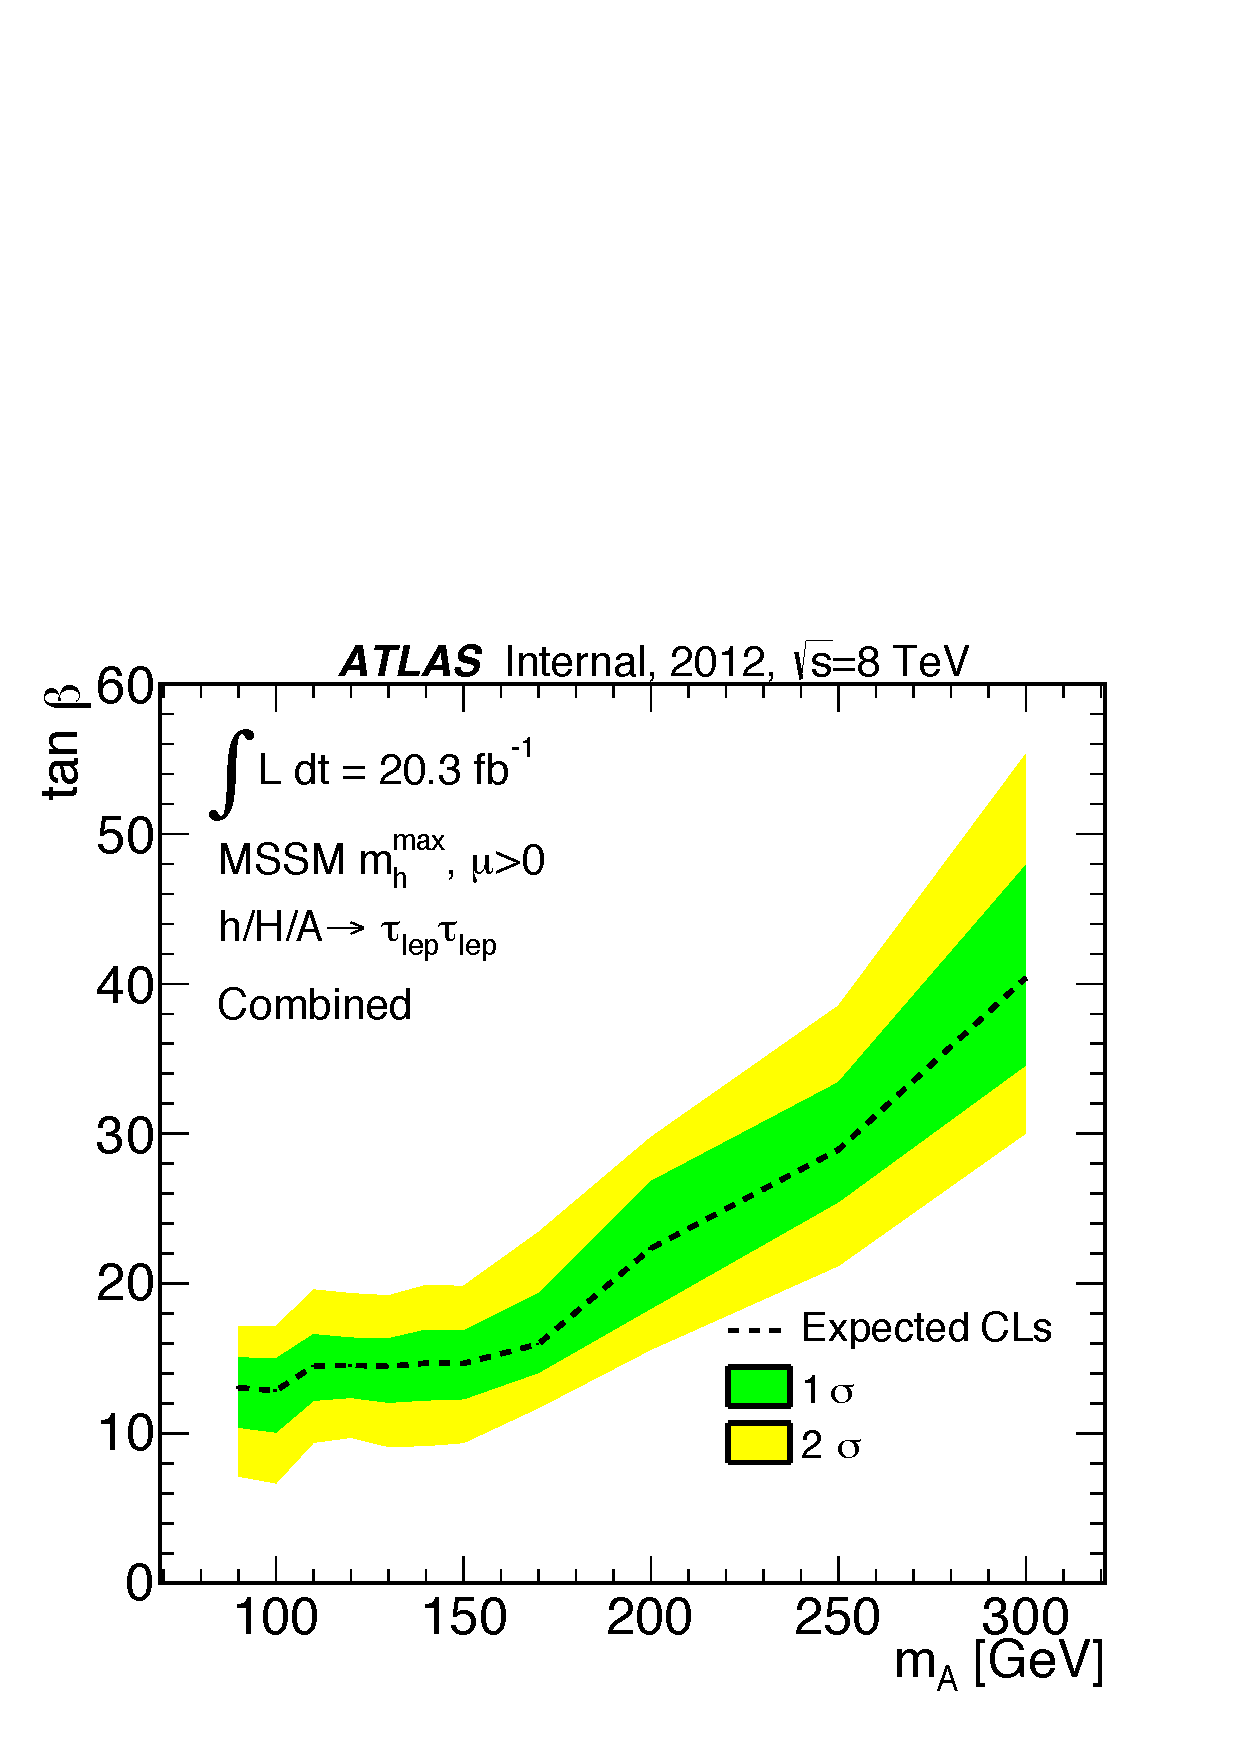
\includegraphics[width=0.65\textwidth]{figure/limits/Limits_mAtanBeta_Comb.pdf}
  \caption{Expected %and observed 
  exclusion limits for MSSM Higgs boson production 
in the MSSM $m_A$ vs $\tan\beta$ parameter space. Combination between b-tag and b-veto category.}
\label{fig:limit_extract_combined}
\end{figure}


The outcome of the search is also interpreted in the generic case of a scalar boson produced in the
$pp \rightarrow gg \rightarrow \phi$ or $pp \rightarrow bb\phi$ mode and decaying to a di-tau pair.
These limits are shown in Figure~\ref{fig:limit_xs} 
for the b-associated  and the gluon-gluon fusion production mechanisms separately.
All signal systematic uncertainties are implemented in the likelihood
for this limit derivation, more information about the limits and their validation can be found in Appendix~\ref{appendix:limit}.

\begin{figure}[tp]
  \centering
% \includegraphics[width=0.45\textwidth]{}
% \includegraphics[width=0.45\textwidth]{}
  \caption{ Limits on the production of a scalar particle decaying to a di-tau pair
    and produced     in association with b quarks (left) or   via gluon-gluon fusion (right). Still not produced...}
\label{fig:limit_xs}
\end{figure}

